\pagebreak
\section{Descrizione Design Pattern}
\label{appendice-pattern}

	\subsection{Chain of Responsibility} % patern comportamentale
	Il \glossario{Chain of Responsibility} è un pattern comportamentale che permette di separare i \emph{sender} dai \emph{receiver} delle richieste. La richiesta attraversa una catena di oggetti per essere intercettata solo quando raggiunge il proprio gestore. Viene utilizzato quando non è possibile determinare staticamente il \emph{receiver} oppure l'insieme di oggetti gestori cambia dinamicamente a runtime. \\ Le richieste vengono dette \emph{implicite} poiché il \emph{sender} non ha alcuna conoscenza sull'identità del ricevente. Per permettere alla richiesta di attraversare la catena e per rimanere \emph{implicita}, ogni \emph{receiver} condivide un interfaccia comune per gestire le richieste ed accedere al proprio successore. 
	La gerarchia che vorrà inviare richieste dovrà avere una superclasse che dichiara un metodo \emph{handler} generico, la specializzazione di tale metodo avviene tramite \emph{overriding} nelle sottoclassi opportune, come illustrato in figura \ref{fig:chainofresponsibility}.
	
	\begin{figure}[h]
	\centering 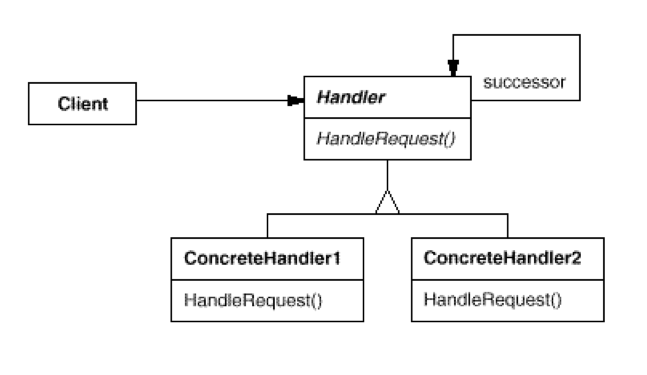
\includegraphics[width=0.7\textwidth]{patterns/ChainOfResponsability.png}
	\caption{Struttura del chain of responsibility.}
	\label{fig:chainofresponsibility}
	\end{figure}
	
	L'utilizzo di questo pattern comporta una serie di conseguenze:
		\begin{itemize}
			\item Ridotto accoppiamento: gli oggetti non sono a conoscenza di chi gestirà la richiesta ma sanno solo che verrà gestita in modo appropriato. Inoltre non bisognerà manutenere i riferimenti a tutti i possibili riceventi;
			\item Aggiunge flessibilità nell'assegnamento delle responsabilità degli oggetti: è possible distribuire le responsabilità tra gli oggetti a runtime modificandone la gerarchia. Staticamente è possibile usare il \emph{subclassing} per specializzare i gestori;
 			\item Non c'è garanzia che la \emph{request} venga gestita, questo può avvenire quando la catena non è stata costruita in modo rigoroso.
		\end{itemize}
	
		
	
	\subsection{Middleware} 
	Il \glossario{Middleware} è uno strato software che si interpone tra l'applicazione software e il sistema operativo per semplificarne le comunicazioni e la gestione di input/output. Viene solitamente utilizzato in applicazioni distribuite e facilita l'interoperabilità fornendo servizi che permettono la comunicazione tra applicazioni di sistemi operativi diversi. La distinzione tra lo strato software del sistema operativo è, per alcune entità, arbitraria, può infatti accedere che il \glossario{Middleware} fornisca dei servizi abitualmente attribuibili a un sistema operativo. I primi utilizzi di \glossario{Middleware} risalgono agli anni '80, come soluzione ai problemi di comunicazione tra applicazioni nuove e meno recenti. 
	
	\begin{figure}[h]
	\centering 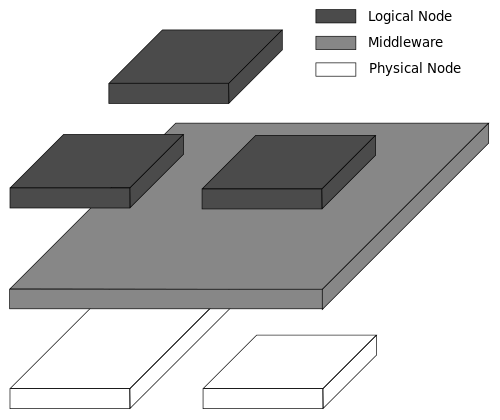
\includegraphics[width=0.7\textwidth]{patterns/Middleware.png}
	\caption{Struttura del middleware.}
	\label{fig:middleware}
	\end{figure}
	
	I servizi \glossario{Middleware} forniscono un set di interfacce che permetto a un applicazione di:
	
	\begin{itemize}
		\item Localizzare facilmente applicazioni o servizi in una rete;
		\item Filtrare dati per renderli user-friendly oppure anonimizzarli per renderli pubblicabili proteggendone la privacy;
		\item Essere indipendente dai servizi di rete;
		\item Essere affidabile e sempre disponibile;
		\item Aggiungere attributi complementari.
	\end{itemize}
	
	Si tratta quindi di funzionalità leggermente più specializzate da quelle normalmente offerte da un sistema operativo. 
	L'avvento del web ha avuto una forte ripercussione sulla diffusione dei software di \glossario{Middleware}, hanno infatti permesso l'accesso sicuro da remoto di database locali.
	I tipi di \glossario{Middleware} sono:
	
	\begin{itemize}
		\item Message-Oriented Middleware (\glossario{MOM}): sono \glossario{Middleware} dove le notifiche degli eventi vengono spedite come messaggi tra sistemi o componenti. I messaggi inviati al client vengono memorizzati fintanto che non vengono gestiti, nel frattempo il client può svolgere altro lavoro;
		\item Enterprise messaging system: è un tipo di \glossario{Middleware} che facilita il passaggio di messaggi tra sistemi diversi o componenti in formato standard, spesso utilizzando servizi web o \glossario{XML};
		\item Message broker: è parte dell \emph{entreprise messaging system}. Accoda, duplica, traduce e spedisce messaggi a sistemi o componenti diverse;
		\item Enterprise Service Bus: è definito come qualche tipo di \glossario{Middleware} integrato che supporta sia \glossario{MOM} che dei servizi web.
		\item Intelligent Middleware: gestisce il processamento in tempo reale di grandi volumi di segnali che trasforma in informazioni di business. Particolarmente adatto per architetture scalabili e distribuite;
		\item Content-Centric Middleware: questo tipo di \glossario{Middleware} fornisce una semplice astrazione con la quale le applicazioni possono inoltrare richieste per contenuti univocamente identificati, senza occuparsi su come e dove vanno ottenuti.
		
	\end{itemize}	 
	
	% possibile add: http://www.networkcomputing.com/netdesign/cdmwdef.htm
	
 	
	
	\subsection{Injection} %angular
	
	\subsection{Singleton} % creazionale
	Il \glossario{Singleton} è un design pattern creazionale che permette di avere un unica istanza di una classe con un unico punto di accesso noto. Tale condizione è tipica di alcuni contesti e trova risvolti pratici in svariate applicazioni. Per permettere l'implementazione di questo pattern è sufficiente che la classe stessa si occupi di tracciare la propria istanziazione e bloccarla qualora sia già avvenuta almeno una volta. Il \glossario{Singleton} dovrebbe essere estensibile usando il \emph{subclassing} il client può utilizzarne l'estensione senza quindi modificarne il codice.
	
		\begin{figure}[h]
	\centering 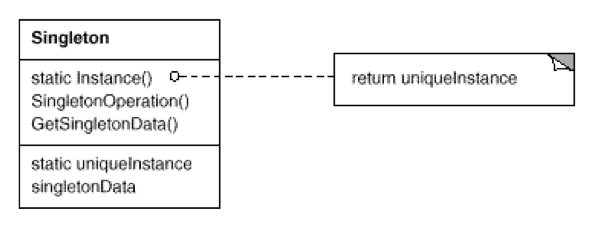
\includegraphics[width=0.7\textwidth]{patterns/Singleton.png}
	\caption{Struttura del singleton.}
	\label{fig:singleton}
	\end{figure}
	
	L'utilizzo di questo pattern comporta una serie di conseguenze:
	\begin{itemize}
		\item Accesso controllato alla singola istanza: poiché la classe \glossario{Singleton} incapsula la sua unica istanza, è in grado di controllare quando e come i client vi accedono;
		\item Namespace pulito: l'utilizzo di questo pattern risulta migliore rispetto all'uso di variabili globali poiché scongiura l'inquinamento del name space globale;
		\item Permette raffinamenti di operazioni e rappresentazioni: il \glossario{Singleton} dovrebbe venire sempre esteso prima dell'utilizzo, che in termini pratici si traduce in un operazione banale, questo può avvenire anche in runtime;
		\item Eventualmente permette un numero variabile di istanze: questo pattern permette, se necessario, di avere istanze multiple mantenendo però il controllo sul numero;
		\item Flessibilità; un modo per avere una funzionalità riconducibile al \glossario{Singleton} è quello di utilizzare le operazioni sulle classi, come per esempio la keyword \code{static} del C++, ma in questo modo è più difficile controllarne il design e permetterne più istanze. Inoltre nel linguaggio succitato le funzioni statiche non sono mai virtuali, rendendone impossibile l'utilizzo polimorfo alle sottoclassi che le ridefiniscono.
	\end{itemize}
	
	\subsection{Registry} %libro dropbox